% ----------------------------------------------------------------------- %
% Arquivo: 5-implementacao.tex
% ----------------------------------------------------------------------- %

\chapter{Implementação do Sistema de Armazenamento Distribuído}
\label{c_implementacao}

A proposta de implementação deste trabalho consiste na criação de um \textit{cluster} Kubernetes e implantação de armazenamento distribuído utilizando a plataforma de armazenamento Rook.

O \textit{cluster} Kubernetes foi criado através da utilização de três máquinas virtuais e uma sub-rede configuradas na \ac{GCP}. A infraestrutura foi criada remotamente na \ac{GCP} utilizando o Terraform, que é uma aplicação para manutenção e gerenciamento de infraestruturas através de código. Escolheu-se a \ac{GCP} para implementação do trabalho devido ao número de créditos de teste disponíveis para utilização na plataforma, mas outros provedores de infraestrutura tais como \ac{AWS} ou \textit{Microsoft Azure} poderiam ter sido utilizados já que o Terraform também suporta a criação de infraestruturas nestes provedores. É importante ressaltar que foram utilizadas máquinas virtuais para que o cenário implementado pudesse ser replicado tanto em outros provedores quanto localmente, não tornando assim a implementação dependente de \ac{API}s ou serviços específicos do provedor, tais como \ac{AKS} ou \ac{Amazon EKS}.

Já o \textit{cluster} Kubernetes foi criado através do Rancher, que é uma ferramenta para gerenciamento de \textit{clusters} Kubernetes. Esta ferramenta permite, por exemplo, a criação automatizada de \textit{clusters} e adição e remoção de nós de processamento ao \textit{cluster}, além de fornecer ferramentas para monitoramento dos serviços implantados. O Rancher já é utilizado no ambiente de produção da infraestrutura de serviços mantida no câmpus do \ac{IFSC} de São José.

Após a criação da infraestrutura necessária e implantação do \textit{cluster} Kubernetes, o Rook foi implantado para gerir o armazenamento do \textit{cluster}, e uma base de dados MySQL e um \textit{blog} WordPress foram instalados para utilização do armazenamento fornecido pelo Rook. Instruções detalhadas sobre a criação da infraestrutura remota e do \textit{cluster} Kubernetes estão disponíveis na seção de Anexos.

% ----------------------------------------------------------------------- %
\section{Criação da infraestrutura remota}

As especificações das máquinas virtuais utilizadas, tais como tipo de máquina utilizada e distribuição Linux instalada estão disponíveis na tabela \autoref{tabela-vms}.
\newline

\begin{table}[htb]
\centering
\caption{Especificação das máquinas virtuais}%
\label{tabela-vms}
\begin{tabular}{ccc}
\toprule
  Especificação & Valor \\
\midrule \midrule
  Tipo de máquina virtual & \textit{n1-standard-2} \\
\midrule
  Número de máquinas virtuais criadas & 3 \\
\midrule 
  Número de \textit{cores} & 2 \ac{vCPUs} \\
\midrule 
  Quantidade de memória RAM & 7.5 GB \\
\midrule
  Tipo de disco rígido & \textit{Standard persistent disk} \\
\midrule
  Quantidade de armazenamento & 15 GB \\
\midrule
  Zona e Região & \textit{southamerica-east1-a} \\
\midrule
  Distribuição Linux & Debian 9 (\textit{Stretch}) \\
\bottomrule
\end{tabular}%
{%
  \fonte{Elaborado pelo autor.}%
}
\end{table}

A sub-rede criada possui regras de \textit{firewall} específicas para permitir que apenas as portas necessárias para funcionamento dos serviços implantados e gerenciamento do \textit{cluster} Kubernetes estejam abertas. A tabela \autoref{tabela-sub-rede} mostra quais portas foram abertas para os protocolos \ac{TCP} e \ac{UDP}.

\begin{table}[htb]
\centering
\caption{Especificação da sub-rede}%
\label{tabela-sub-rede}
\begin{tabular}{ccc}
\toprule
  Especificação & Valor \\
\midrule \midrule
  Faixa de \ac{IP}s & 10.0.0.0/24 \\
\midrule 
  Tipo de endereço & Interno \\
\midrule 
  Portas de \textit{firewall} abertas para protocolo \ac{TCP} & 22, 53, 80, 443, 2380, 2379, 3306, \\
  & 6443, 6970, 6800-7300, 8124, 9283, \\
  & 10250, 10254, 30000-32767, 44134 \\
\midrule
  Portas de \textit{firewall} abertas para protocolo \ac{UDP} & 53, 8472 \\
\bottomrule
\end{tabular}%
{%
  \fonte{Elaborado pelo autor.}%
}
\end{table}

A criação da infraestrutura remota foi realizada utilizando o Terraform, que permite que componentes da infraestrutura sejam descritos como código e gerenciados através do \textit{software}. O \autoref{l_terraform-vm} mostra um trecho do código utilizado para criação de uma das máquinas virtuais utilizadas no projeto através do Terraform.

\begin{lstlisting}[language=Caml,caption=Configuração de máquina virtual descrita no arquivo de configuração do Terraform,captionpos=t,label=l_terraform-vm, numbers=none]
resource "google_compute_instance" "vm-0" {
  name         = "vm-0"
  machine_type = "n1-standard-2"
  zone         = "southamerica-east1-a"

  boot_disk {
    initialize_params {
      image = "debian-cloud/debian-9"
      size = "15"
    }
  }

  network_interface {
    subnetwork    = "${google_compute_subnetwork.subnet-0.name}"
    address       = "${google_compute_address.address-0.address}"
    access_config = {}
  }

  metadata {
    sshKeys = "${var.gce_ssh_user}:${file(var.gce_ssh_pub_key_file)}"
  }

  metadata_startup_script = "${data.template_file.startup_script.rendered}"

  tags = ["k8s"]
}
\end{lstlisting}

A sintaxe da configuração é: o recurso criado é do tipo \texttt{google\_compute\_instance} (máquina virtual) e nomeado como \texttt{vm-0}. A máquina virtual é do tipo predefinido \texttt{n1-standard-2} e localizada na zona e região \texttt{southamerica-east1-a} (São Paulo). O disco de inicialização da máquina terá armazenamento de \texttt{15 GB} e será instalada a imagem da distribuição linux \texttt{debian-cloud/debian-9}. O nome da rede ao qual a máquina será associada está definido no parâmetro \texttt{google\_compute\_subnetwork.subnet-0.name} e endereço de rede interno será o definido no parâmetro \texttt{google\_compute\_address.address-0.address}. O nome do usuário criado na máquina virtual será o armazenado na variável \texttt{var.gce\_ssh\_user} e suas chaves para acesso através \ac{SSH} estão disponíveis no arquivo referenciado pela variável \texttt{var.gce\_ssh\_pub\_key\_file}. Também será adicionado um \texttt{script} de inicialização a ser executado toda vez que a máquina for iniciada, o qual está definido em \texttt{data.template\_file.startup\_script.rendered}. Este \textit{script} está disponível no \autoref{l_startupscript_file}. Também será adicionada à máquina virtual uma \textit{tag} de valor \texttt{k8s}. O arquivo completo utilizado para criação de toda a infraestrutura está disponível no \autoref{l_terraform_file}.

Após a descrição dos componentes da infraestrutura necessários no formato aceito pelo Terraform a infraestrutura remota foi criada na \ac{GCP}. A \autoref{gcp_vms} mostra as máquinas virtuais criadas através do Terraform na \ac{GCP}.

\begin{figure}[!htpb]
	\centering
	\caption{Máquinas virtuais criadas na \ac{GCP}}
    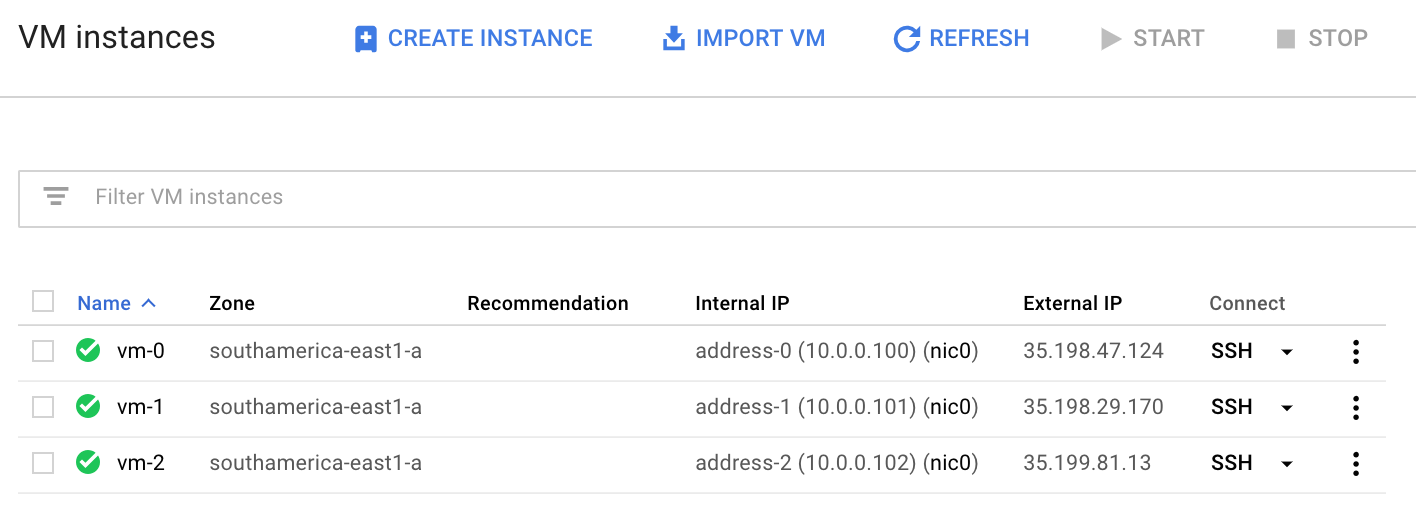
\includegraphics[width=16cm]{TCC/figuras/5-implementacao/vms}
    
	Fonte: Elaborado pelo autor.
 	\label{gcp_vms}
\end{figure}

% ----------------------------------------------------------------------- %
\section{Criação do \textit{cluster} Kubernetes}

Para criação do \textit{cluster} Kubernetes remoto foi utilizado o Rancher, que é uma ferramenta para gerenciamento de \textit{clusters} Kubernetes. Os únicos requisitos para criação do \textit{cluster} remoto utilizando o Rancher são de que os dispositivos que farão parte do \textit{cluster} possuam versões do \texttt{Docker} instalado compatíveis com a versão do Rancher utilizada e que sejam fornecidas ao Rancher chaves \ac{SSH} de um usuário que possua privilégios de administrador. Assim, os componentes necessários, como contêineres, serão automaticamente instalados e o \textit{cluster} Kubernetes criado. Escolheu-se utilizar o Rancher por dois motivos principais, sendo o primeiro a vantajosa automatização da criação do \textit{cluster} (que pode ser complexa devido as configurações de rede) e o segundo a independência de plataforma que o Rancher oferece, podendo ser utilizado para gerenciar tanto um \textit{cluster} remoto hospedado em diferentes provedores de \ac{IaaS}/\ac{PaaS} ou local.

Após a instalação do docker nas máquinas virtuais (procedimento automaticamente realizado na criação das máquinas virtuais através de um \textit{script} de inicialização) é necessário dar permissão de execução do comando \texttt{docker} ao usuário na máquina virtual. Assim, as credenciais de acesso deste usuário poderão ser utilizadas pelo Rancher para criar e configurar o \textit{cluster} Kubernetes remoto através do docker instalado nas máquinas. Parte do arquivo de configuração do Rancher utilizado nesta etapa é mostrado no \autoref{l_rancher_master}, enquanto o arquivo completo de configuração pode ser visto no \autoref{l_rancher_file}.
\newline

\begin{lstlisting}[language=Caml,caption=Configuração de nó mestre do \textit{cluster} criado com Rancher,captionpos=t,label=l_rancher_master, numbers=none]
nodes:
- address: 35.198.47.124
  internal_address: 10.0.0.100
  user: matuzalemmuller
  ssh_key_path: keys/id_rsa
  role: [controlplane,worker,etcd]
  hostname_override: master
  labels:
    node: master
}
\end{lstlisting}

Uma breve explicação sobre cada parâmetro utilizado na configuração está disponível abaixo:

\begin{itemize}
    \item \texttt{address}: endereço \ac{IP} público da máquina virtual.
    \item \texttt{internal\_address}: endereço \ac{IP} da máquina virtual na sub-rede na qual ela se encontra.
    \item \texttt{user}: usuário que será utilizado para criação do \textit{cluster}. É necessário que este usuário possua permissões de execução do \texttt{docker} e outras permissões de administrador para que o \textit{cluster} seja criado.
    \item \texttt{ssh\_key\_path}: localização das chaves \ac{SSH} do usuário utilizado no parâmetro \texttt{user} (neste caso, \texttt{matuzalemmuller}).
    \item \texttt{role}: funções do nó no \textit{cluster}. Como este será o nó mestre ele assumirá as funções de \texttt{controlplane} (\textit{master}), \texttt{worker} (executa \textit{pods}) e \texttt{etcd} (armazena as chaves-valor (\textit{key-value}) e estado de aplicações de forma distribuída).
    \item \texttt{hostname\_override}: ignora o nome da máquina virtual e utiliza um nome específico (\texttt{master}) para se referenciar a este nó.
    \item \texttt{labels}: é adicionado um \texttt{label} de valor \texttt{master} para que \textit{pods} possam ser criados especificamente neste nó ao referenciar este \texttt{label}, por exemplo.
\end{itemize}

A \autoref{k8s_nodes} mostra o \textit{cluster} disponível após sua criação com os três nós do \textit{cluster} Kubernetes em execução. A ferramenta de linha de comando \texttt{kubectl} é utilizada para gerenciamento do \textit{cluster} Kubernetes.

\begin{figure}[!htpb]
    \centering
    \caption{Saída do terminal: Nós em execução após criação de \textit{cluster} com Rancher}
\begin{verbatim}
    matuzalem-macbook:remote-setup matuzalem$ kubectl get node
    NAME      STATUS    ROLES                      AGE       VERSION
    master    Ready     controlplane,etcd,worker   1m        v1.11.1
    worker1   Ready     etcd,worker                1m        v1.11.1
    worker2   Ready     etcd,worker                1m        v1.11.1
\end{verbatim}
	Fonte: Elaborado pelo autor.
 	\label{k8s_nodes}
\end{figure}

Após a criação do \textit{cluster} um arquivo de nome \texttt{kube\_config\_cluster.yml} será criado. Este arquivo de configuração permite que o \textit{cluster} seja acessado e gerenciado externamente.

% ----------------------------------------------------------------------- %
\section{Implantação do Rook para utilização de armazenamento}

Após a criação da infraestrutura e do \textit{cluster} Kubernetes é possível instalar o Rook para que seja realizada a gestão de armazenamento no \textit{cluster}. 

A instalação do Rook consiste em três procedimentos principais, sendo o primeiro a instalação do Rook no \textit{cluster} para criação de operadores e agentes nos nós. Isto permitirá que o Ceph seja iniciado nos nós, mas nenhum disco será mapeado ainda. Para que os discos sejam mapeados pelo Rook (e consequentemente pelo Ceph) é necessário criar o \textit{cluster} Rook. Este \textit{cluster} irá criar \textit{pods} adicionais em cada nó, que consistem em \textit{monitors} e \ac{OSD}s, além do \textit{operator} criado no nó mestre. Um \textit{operator} é, de forma simples, um recurso utilizado para permitir que sejam implantados \ac{CRD}s e ciclos de automatização de tarefas ao implantar aplicações, não sendo necessário criar estas funcionalidades ao implantar as aplicações \cite{coreosoperators}. Após a instalação do Rook e criação do \textit{cluster} para mapeamento dos discos é possível utilizar o Rook para prover armazenamento. A \autoref{rook_architecture} demonstra uma arquitetura do Rook que contempla todos os tipos de armazenamento disponíveis e os componentes utilizados para prover o armazenamento.

\begin{figure}[!htpb]
	\centering
	\caption{Representação da arquitetura do Rook}
    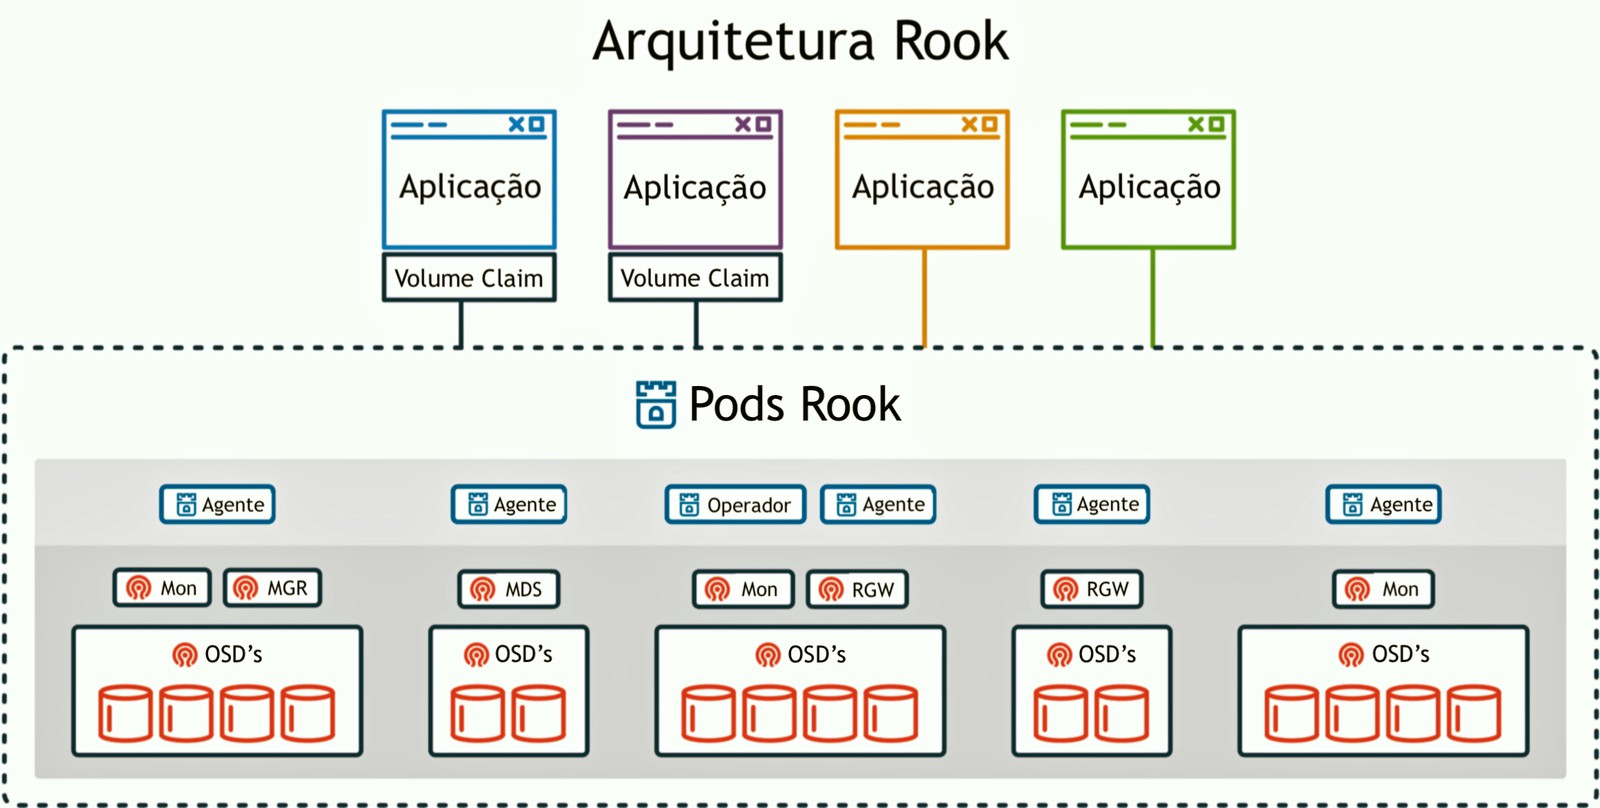
\includegraphics[width=16cm]{TCC/figuras/5-implementacao/Rook_Architecture}
    
	Fonte: Traduzido de \cite{aboutrook}.
 	\label{rook_architecture}
\end{figure}


Os componentes criados pelo Rook são diretamente equivalentes aos componentes do Ceph. Isto significa, por exemplo, que um \textit{monitor} do Rook é a implementação do \textit{monitor} do Ceph no \textit{cluster} Kubernetes. O mesmo é valido para Agentes, Operadores, \ac{OSD}s, \ac{MDS}s e \ac{RGW}s. Já as \textit{Volume Claims} representam requisições das aplicações para o \textit{cluster}, requisitando um volume para armazenamento de dados.

Em termos de implementação, o Rook \textit{operator}, que consiste nos operadores e agentes do Rook, pode ser instalado no \textit{cluster} através do Helm. Neste trabalho a versão utilizada do Rook foi a \textit{release} versão 0.8.0, a qual possui a implementação do Ceph em estado beta. Como há um mestre e dois nós no \textit{cluster} Kubernetes, serão criados no \textit{namespace} \texttt{rook-ceph-system} três \textit{pods} de \textit{agents}, um em cada nó. Além destes \textit{pods} também serão criados \textit{discovers} (responsáveis por identificar os dispositivos disponíveis para armazenamento nas máquinas virtuais) e um \textit{operator}, sendo o último disponível apenas no nó mestre. A \autoref{rook_operator_pods} mostra os componentes criados no \textit{namespace} \texttt{rook-ceph-system}.

\begin{figure}[!htpb]
	\centering
	\caption{Saída do terminal: \textit{Pods} criados pelo Rook \textit{Operator}}
    \begin{verbatim}
matuzalem-macbook:rook matuzalem$ kubectl get pod -n rook-ceph-system
NAME                                  READY     STATUS    RESTARTS   AGE
rook-ceph-agent-j7vkn                 1/1       Running   0          1m
rook-ceph-agent-lgzqm                 1/1       Running   0          1m
rook-ceph-agent-sngjz                 1/1       Running   0          1m
rook-ceph-operator-59c6b78b7c-lsz2l   1/1       Running   0          1m
rook-discover-67t94                   1/1       Running   0          1m
rook-discover-b69j4                   1/1       Running   0          1m
rook-discover-ljzqv                   1/1       Running   0          1m
    \end{verbatim}
	Fonte: Elaborado pelo autor.
 	\label{rook_operator_pods}
\end{figure}

Após realizar a inicialização do Rook \textit{operator} é possível criar o \textit{cluster} Rook. A criação do \textit{cluster} foi manualmente realizada utilizando o código disponível no \autoref{l_rook-cluster_file}. Este código cria o \textit{cluster}, \textit{namespace} e outros componentes necessários para a utilização do Rook. Neste caso os principais componentes criados serão um \textit{pod} \textit{manager}, três \textit{pods} de \textit{monitors} e três \textit{pods} de \ac{OSD}s, os quais são criados no \textit{namespace} \texttt{rook-ceph}. A \autoref{rook_cluster_pods} mostra os pods criados em execução no \textit{cluster} Rook.

\begin{figure}[!htpb]
	\centering
	\caption{Saída do terminal: \textit{Pods} criados pelo \textit{Cluster} Rook}
    \begin{verbatim}
matuzalem-macbook:rook matuzalem$ kubectl get pod -n rook-ceph
NAME                                  READY     STATUS      RESTARTS   AGE
rook-ceph-mgr-a-7944d8d79b-sjfxw      1/1       Running     0          3m
rook-ceph-mon0-5qj7l                  1/1       Running     0          4m
rook-ceph-mon1-rfvpj                  1/1       Running     0          4m
rook-ceph-mon2-xc966                  1/1       Running     0          4m
rook-ceph-osd-id-0-6cdfc557f-n6hdk    1/1       Running     0          3m
rook-ceph-osd-id-1-5475fbb74-wbh74    1/1       Running     0          3m
rook-ceph-osd-id-2-5f68f97d4d-87hpx   1/1       Running     0          3m
rook-ceph-osd-prepare-master-7dbhx    0/1       Completed   0          3m
rook-ceph-osd-prepare-worker1-cwzf7   0/1       Completed   0          3m
rook-ceph-osd-prepare-worker2-cqbc2   0/1       Completed   0          3m
    \end{verbatim}
	Fonte: Elaborado pelo autor.
 	\label{rook_cluster_pods}
\end{figure}

Agora que o \textit{cluster} Rook foi criado é possível configurá-lo para utilizá-lo para prover o armazenamento de objetos, blocos ou arquivos. Neste trabalho os tipos de armazenamento utilizados serão blocos e objetos.

O armazenamento em blocos será utilizado para gestão de volumes persistentes a serem utilizados por contêineres, os quais persistem dados após seu reinício. Isto permite, por exemplo, que os contêineres não percam suas configurações ou estados. Esta é uma boa forma de armazenar configurações e conteúdos que são frequentemente modificados por contêineres. Já o armazenamento através de objetos será utilizado para armazenar e distribuir conteúdos estáticos, tais como imagens e arquivos que são pouco modificados.

O armazenamento em blocos pode ser implementado no Rook através de um \textit{StorageClass}, enquanto o armazenamento de objetos é disponibilizado através de uma \textit{Object Store}. Ambos serão explicados nos parágrafos seguintes.

Para a configuração do armazenamento de dados através de objetos é necessário criar um \textit{StorageClass} específico do Rook. A criação deste \textit{StorageClass} é realizado utilizando o código disponível no \autoref{l_rook-storage-class_file}. Após a criação deste \textit{StorageClass} volumes persistentes (\ac{PV}) poderão ser criados através de requisições de volumes (\ac{PVC}) ao Rook.

Já para o armazenamento de objetos no \textit{cluster} Rook é necessário que uma \textit{Object Store} seja criada. Uma \textit{Object Store} é um \ac{CRD} criado pelo Rook e possui como função criar os componentes necessários para gerenciamento dos objetos no \ac{RADOS} do Ceph, fornecendo assim acesso a estes objetos através de um \textit{pod} equivalente ao \ac{RADOS} \textit{Gateway}. Assim como o \ac{RADOS} \textit{Gateway} oferece uma \ac{REST} \ac{API} de acesso compatível com a interface S3 da Amazon aos objetos armazenados, o \textit{cluster} Rook também permite que arquivos sejam gerenciados através desta \ac{API}. Logo, é possível criar \textit{buckets} no \textit{cluster} Rook, os quais serão utilizados para armazenar dados estáticos e publicamente acessíveis. Neste trabalho um domínio \texttt{.cc} foi utilizado para validação do modelo, utilizando assim o balanceamento de carga de requisições \ac{HTTP} também através de \ac{DNS}.

A \autoref{rook_rgw_pod} mostra o \textit{pod} criado para execução do \ac{RADOS} \textit{gateway} no \textit{cluster} Rook, juntamente com os outros \textit{pods} disponíveis no namespace \texttt{rook-ceph}.

\begin{figure}[!htpb]
	\centering
	\caption{Saída do terminal: \textit{Pod} \ac{RADOS} \textit{Gateway} em execução}
    \begin{verbatim}
matuzalem-macbook:rook matuzalem$ kubectl get pod -n rook-ceph
NAME                                     READY   STATUS     RESTARTS  AGE
rook-ceph-mgr-a-7944d8d79b-sjfxw         1/1     Running    0         10m
rook-ceph-mon0-5qj7l                     1/1     Running    0         11m
rook-ceph-mon1-rfvpj                     1/1     Running    0         11m
rook-ceph-mon2-xc966                     1/1     Running    0         10m
rook-ceph-osd-id-0-6cdfc557f-n6hdk       1/1     Running    0         10m
rook-ceph-osd-id-1-5475fbb74-wbh74       1/1     Running    0         10m
rook-ceph-osd-id-2-5f68f97d4d-87hpx      1/1     Running    0         10m
rook-ceph-osd-prepare-master-7dbhx       0/1     Completed  0         10m
rook-ceph-osd-prepare-worker1-cwzf7      0/1     Completed  0         10m
rook-ceph-osd-prepare-worker2-cqbc2      0/1     Completed  0         10m
rook-ceph-rgw-my-store-fdd764948-vb7fx   1/1     Running    0         13s
    \end{verbatim}
	Fonte: Elaborado pelo autor.
 	\label{rook_rgw_pod}
\end{figure}

% ----------------------------------------------------------------------- %
\section{Implantação de serviços para utilizar armazenamento}

Para utilização do armazenamento foram implantados uma base dados MySQL e um \textit{blog} WordPress. A base de dados é necessária para o funcionamento do \textit{blog} WordPress. A base de dados MySQL utiliza armazenamento em blocos na forma de volumes, enquanto o \textit{blog} WordPress utiliza armazenamento tanto na forma de objetos quanto em blocos. A seguir serão descritas as implementações destes serviços na nuvem remota.

\subsection{MySQL}

A implementação da base de dados MySQL foi realizada através da instalação do serviço pelo Helm. Como é utilizado um gerenciador de pacotes para realizar a instalação da base de dados a sua implantação é rápida e automatizada.

Para utilização do armazenamento em blocos o \textit{pod} MySQL realiza uma \ac{PVC} ao Rook, ou seja, o \textit{pod} solicita a criação de um volume de dados persistentes (\ac{PV}) ao Rook para que este volume seja utilizado como um bloco de armazenamento. O Rook, por sua vez, fornece ao \textit{pod} MySQL o volume requisitado. A \autoref{mysql_pvc_pv} mostra a requisição do volume (\ac{PVC}) realizada pelo \textit{pod} MySQL e o volume (\ac{PV}) entrege ao \textit{pod} pelo Rook.

\begin{figure}[!htpb]
	\centering
	\caption{Saída parcial do terminal: Requisição de volume e volume utilizado pelo \textit{pod} MySQL}
    \begin{verbatim}
matuzalem-macbook:tcc-engtelecom matuzalem$ kubectl get pvc
NAME      STATUS    VOLUME                                    CAPACITY
mysql     Bound     pvc-c3428e0b-f66b-11e8-939f-42010a000064  5Gi      
matuzalem-macbook:tcc-engtelecom matuzalem$ kubectl get pv
NAME                                      CAPACITY  STORAGECLASS
pvc-c3428e0b-f66b-11e8-939f-42010a000064  5Gi       rook-ceph-block
    \end{verbatim}
	Fonte: Elaborado pelo autor.
 	\label{mysql_pvc_pv}
\end{figure}

A \autoref{mysql_pod} mostra o \textit{pod} MySQL em execução, poucos momentos após sua criação.

\begin{figure}[!htpb]
	\centering
	\caption{Saída do terminal: \textit{Pod} MySQL em execução}
    \begin{verbatim}
matuzalem-macbook:tcc-engtelecom matuzalem$ kubectl get pod
NAME                                     READY     STATUS    RESTARTS   AGE
mysql-56655cb669-2zgvc                   1/1       Running   0          3m
    \end{verbatim}
    
	Fonte: Elaborado pelo autor.
 	\label{mysql_pod}
\end{figure}

\subsection{WordPress}

A implementação do WordPress também foi realizada através do Helm, ou seja, o serviço foi rapidamente criado no \textit{cluster} Kubernetes e o Rook foi utilizado para gerir o armazenamento utilizado pelo WordPress. Assim como no \textit{pod} MySQL, um volume também foi criado e associado ao \textit{pod} WordPress através de uma \ac{PVC}. Ambos volume e requisição são mostrados na \autoref{apps_pvc_pv}, juntamente com o volume e requisição do serviço MySQL.

\begin{figure}[!htpb]
	\centering
	\caption{Saída parcial do terminal: Requisição de volume e volume utilizado pelo \textit{pod} WordPress}
    \begin{verbatim}
matuzalem-macbook:tcc-engtelecom matuzalem$ kubectl get pvc
NAME        STATUS    VOLUME                                     CAPACITY
mysql       Bound     pvc-c3428e0b-f66b-11e8-939f-42010a000064   5Gi
wordpress   Bound     pvc-f035bafe-f66c-11e8-939f-42010a000064   5Gi
matuzalem-macbook:tcc-engtelecom matuzalem$ kubectl get pv
NAME                                       CAPACITY   STORAGECLASS
pvc-c3428e0b-f66b-11e8-939f-42010a000064   5Gi        rook-ceph-block
pvc-f035bafe-f66c-11e8-939f-42010a000064   5Gi        rook-ceph-block
    \end{verbatim}
	Fonte: Elaborado pelo autor.
 	\label{apps_pvc_pv}
\end{figure}

A \autoref{wordpress_pod} mostra que o \textit{pod} WordPress também está em execução. É possível perceber que há quatro \textit{pods} em execução no \textit{namespace} \texttt{default}: um do MySQL, outro do WordPress e dois referentes ao NGINX \textit{controller}. Os \textit{pods} do NGINX funcionam como controladores \textit{Ingress} para que o serviço WordPress possa ser acessado externamente. O NGINX pode ser instalado através do Helm e a interação entre os serviços NGINX e WordPress ocorre automaticamente, ou seja, ao instalar o WordPress ele pode ser automaticamente configurado para ser acessado através do NGINX.

\begin{figure}[!htpb]
	\centering
	\caption{Saída do terminal: \textit{Pod} WordPress em execução}
    \begin{verbatim}
matuzalem-macbook:tcc-engtelecom matuzalem$ kubectl get pod
NAME                                                  READY     STATUS   AGE
mysql-56655cb669-2zgvc                                1/1       Running  13m
nginx-nginx-ingress-controller-7dd6474678-5jkqs       1/1       Running  24m
nginx-nginx-ingress-default-backend-5b88698ddc-zc242  1/1       Running  24m
wordpress-wordpress-5fb9cdfcfd-nr7rt                  1/1       Running  5m
    \end{verbatim}
	Fonte: Elaborado pelo autor.
 	\label{wordpress_pod}
\end{figure}

A \autoref{wordpress_blog} mostra a página \textit{web} do \textit{blog} WordPress em execução.

\begin{figure}[!htpb]
	\centering
	\caption{\textit{Blog} WordPress}
    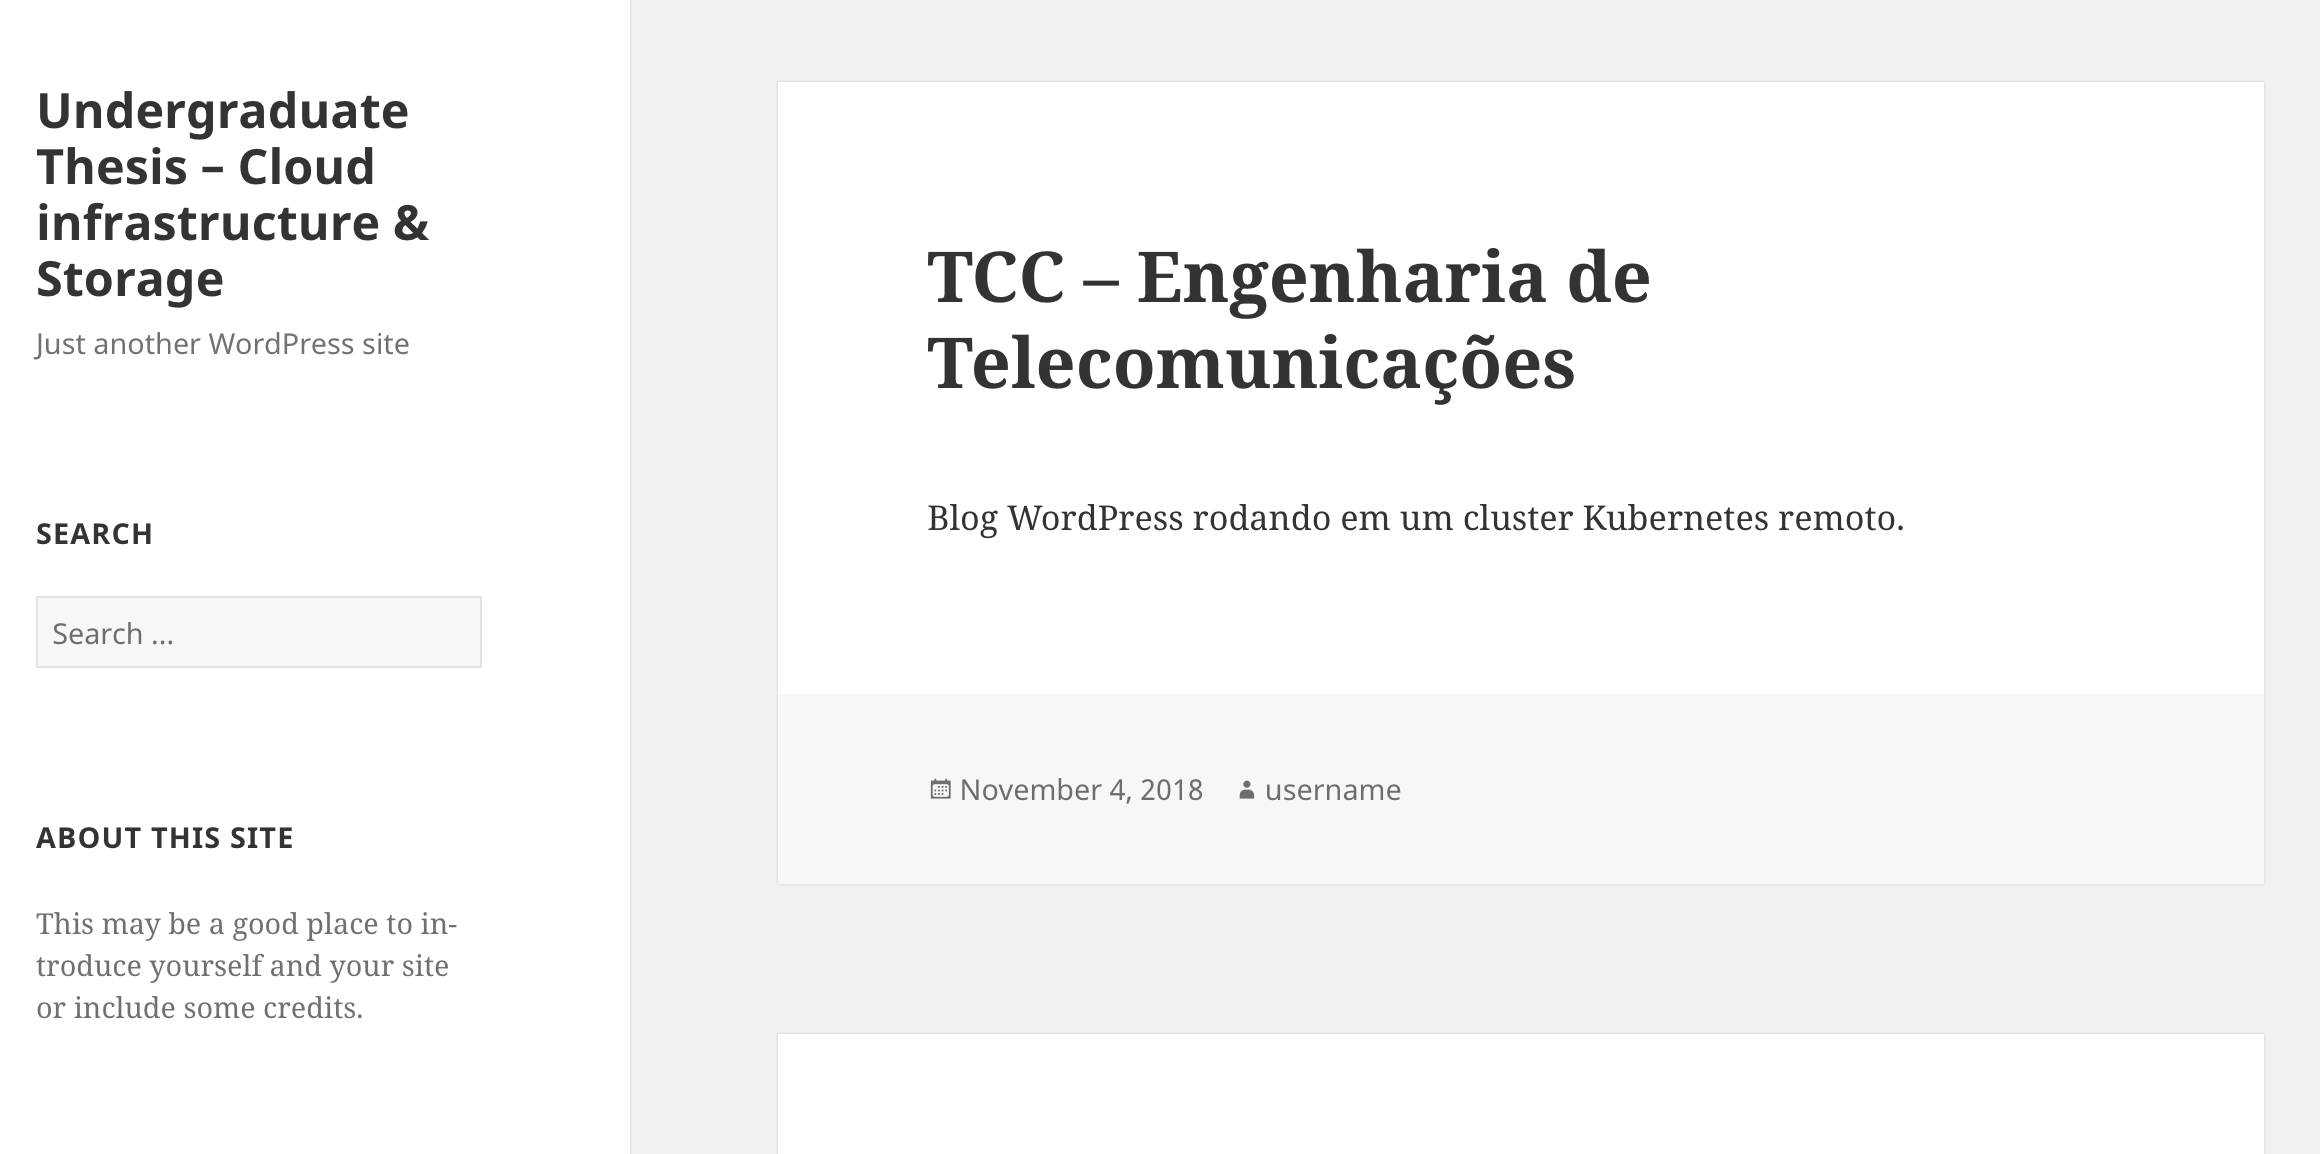
\includegraphics[width=16cm]{TCC/figuras/5-implementacao/wordpress-blog}
    
	Fonte: Elaborado pelo autor.
 	\label{wordpress_blog}
\end{figure}

Até esta etapa o Rook está sendo utilizado para prover armazenamento através de volumes requisitados pelos serviços implantados. Isto significa que o armazenamento utilizado é em blocos, e o armazenamento de objetos ainda não foi utilizado.

Para utilizar o armazenamento de objetos da forma proposta é necessário armazenar objetos na \textit{Object Store} do Rook e tornar estes objetos publicamente acessíveis. Neste trabalho uma imagem será salva como um objeto na \textit{Object Store} do Rook e ela será utilizada pelo WordPress no \textit{blog}. Para isto, é necessário criar um usuário no \ac{RADOS} \textit{gateway} e utilizar este usuário para criar um \textit{bucket} e administrar o armazenamento dos objetos. Após a criação do usuário e \textit{bucket} é possível armazenar uma imagem como objeto na \textit{Object Store}. A imagem utilizada neste projeto é a da \autoref{object_image}. Esta imagem não possui direitos autorais, é do tipo \texttt{jpg} e possui 179 KB.

\begin{figure}[!htpb]
	\centering
	\caption{Imagem armazenada como objeto}
    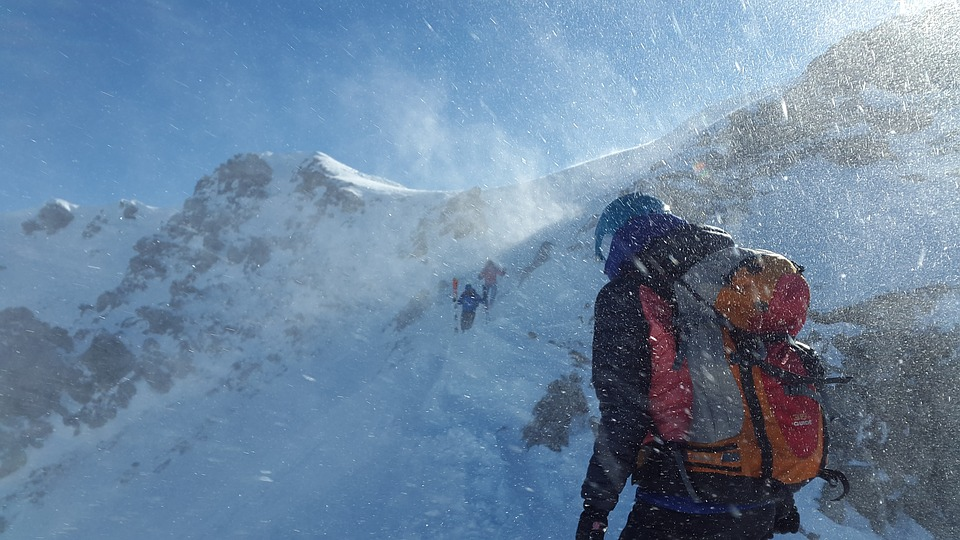
\includegraphics[width=15cm]{TCC/figuras/5-implementacao/example-image}
    
	Fonte: \cite{image}
 	\label{object_image}
\end{figure}

Agora que a imagem está armazenada como um objeto é necessário torna-lá publica, o que pode ser feito através da utilização do \textit{Ingress} NGINX. O código utilizado para implantar o recurso \textit{ingress} está disponível no \autoref{l_rook-object_ingress_file}. 

Com a imagem publicada é possível utilizá-la no WordPress. A \autoref{wordpress_post} mostra a utilização da imagem em uma publicação no WordPress.

\begin{figure}[!htpb]
	\centering
	\caption{Publicação WordPress utilizando imagem armazenada como objeto}
    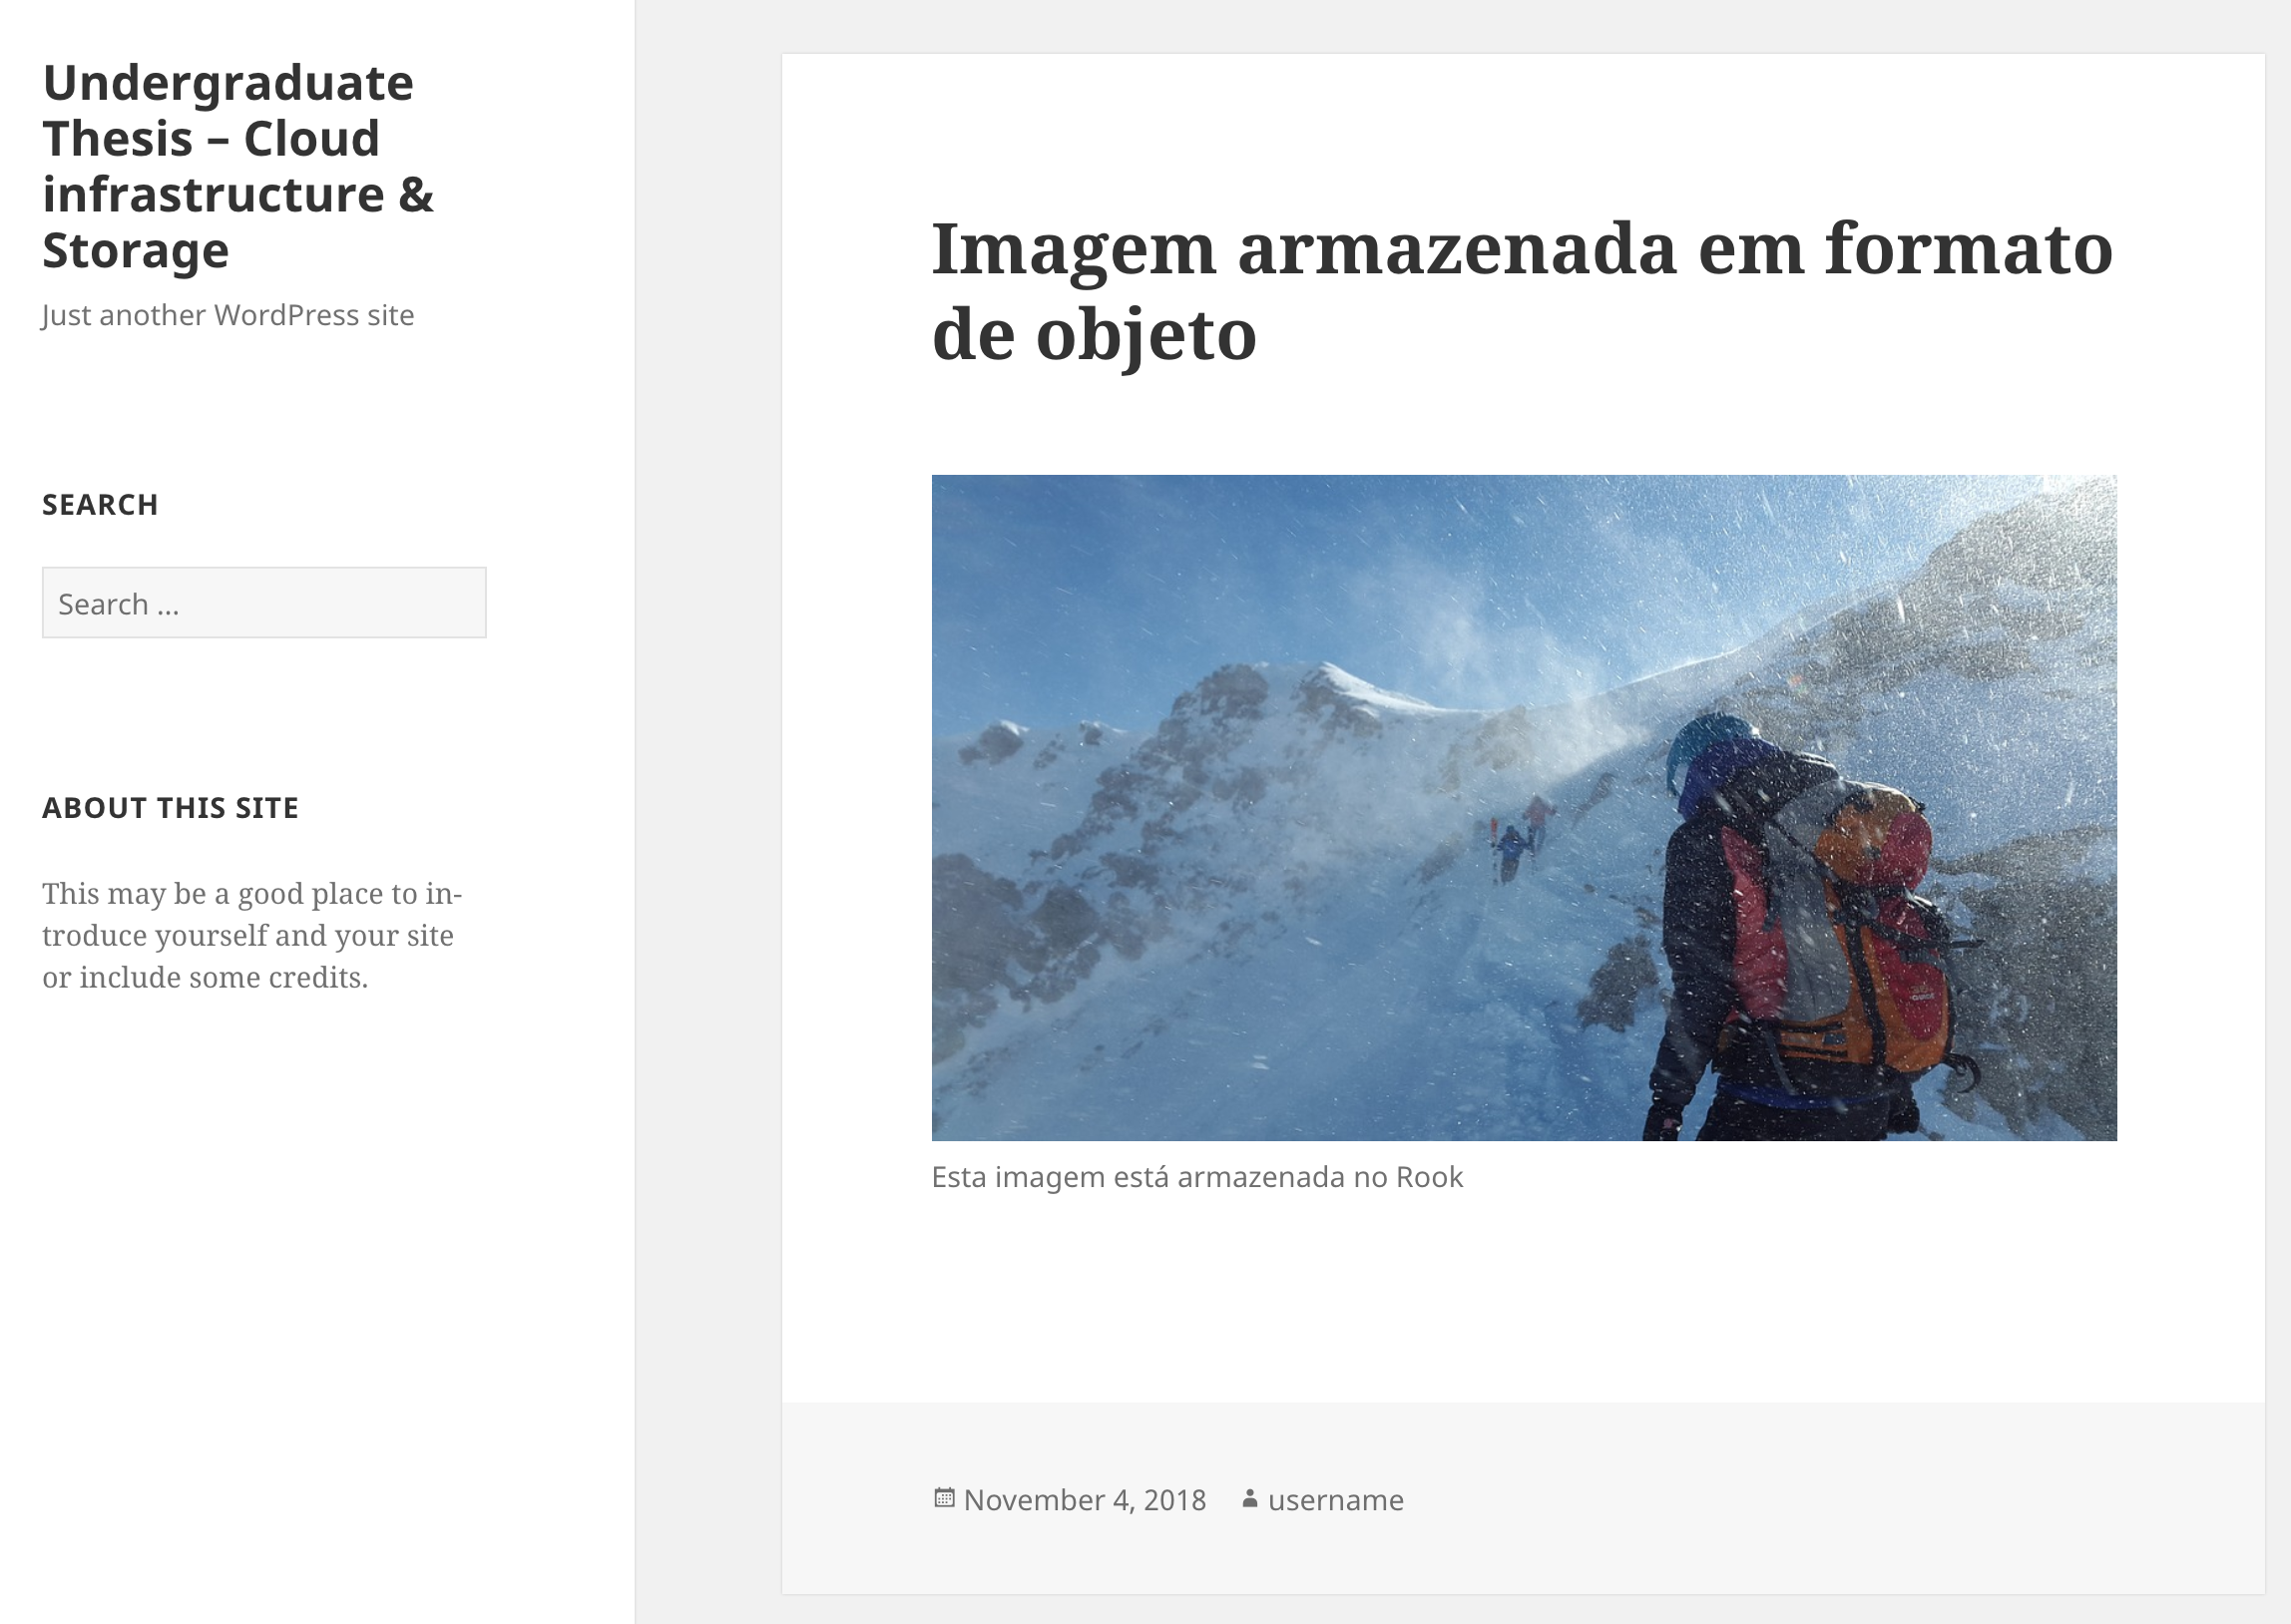
\includegraphics[width=15cm]{TCC/figuras/5-implementacao/wordpress-post}
    
	Fonte: Elaborado pelo autor.
 	\label{wordpress_post}
\end{figure}

A \autoref{wordpress_mysql_schematic} é um diagrama geral da implementação realizada neste trabalho. Os objetos \texttt{Deploment}, \texttt{ReplicaSet}, \texttt{MySQL Pod} e \texttt{WordPress Pod} são automaticamente criados através da instalação de \textit{charts} disponíveis no Helm. As \ac{PVC} são realizadas ao \texttt{StorageClass}, que cria volumes (\ac{PV}) a serem utilizados pelos \texttt{Pods}. Já o objeto \texttt{RGW} é criado através da \textit{Object Store} do Rook. É importante ressaltar que ambos o \texttt{StorageClass} e \texttt{RGW} são \ac{CRD}s do Rook e utilizam o Ceph para armazenamento dos dados. O \texttt{Ingress Controller}, por sua vez, é configurado por objetos \textit{Ingress} automaticamente criados pelas aplicações. A automatização na implantação de serviços e gerenciamento dos recursos comprova a facilidade de utilização do Kubernetes, além de sua eficácia em fornecer uma única plataforma de gerenciamento que combina rede, armazenamento e computação, caracterizando assim este modelo como uma infraestrutura hiperconvergente.

\begin{figure}[!htpb]
	\centering
	\caption{Esquemático da implementação}
    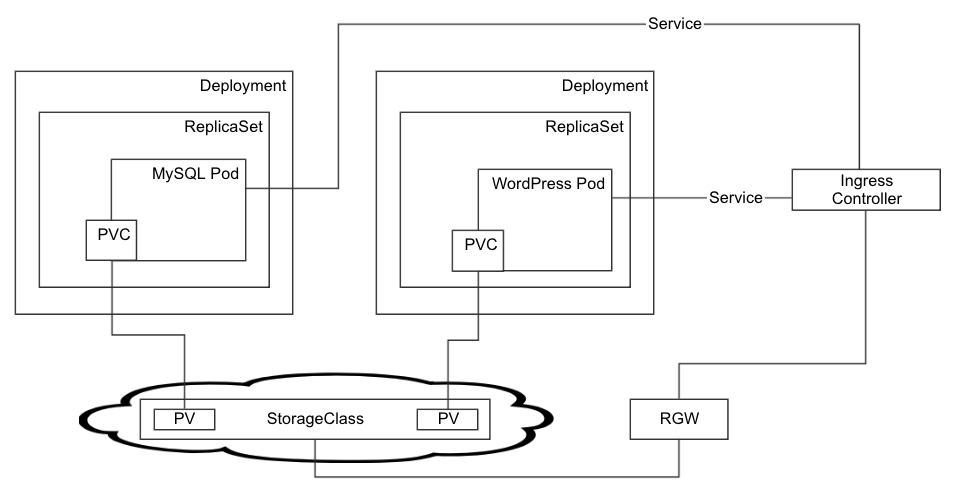
\includegraphics[height=7cm]{TCC/figuras/5-implementacao/apps-schematic.png}
    
	Fonte: Elaborado pelo autor.
 	\label{wordpress_mysql_schematic}
\end{figure}